\documentclass[
	ngerman,
	%twoside,
	BCOR=8mm,
	headings=normal,
	parskip=half,
	headsepline,
	automark,
	listof=totoc,
	bibliography=totoc,
	%,captions=tableabove
	%draft
]{scrreprt}
%
%
\input{packages}
%
\input{definitions}
%
%%%%%%%%%%%%%%%%%%%%%%%%%%%%%%%%%%%%%%%%%%%%%%%%%%%%%%%%%%%%%%%%%%%%%%%%%%%%%%%
% Begriffe für glossaries definieren
%%%%%%%%%%%%%%%%%%%%%%%%%%%%%%%%%%%%%%%%%%%%%%%%%%%%%%%%%%%%%%%%%%%%%%%%%%%%%%%

%=== Glossar ==================================================================
\newglossaryentry{git}{
	name={Git},
	description={Ein kostenloses Versionsverwaltungssystem, entwickelt von Linus Torvald.}
}

\newglossaryentry{github}{
	name={GitHub},
	description={Eine Entwickler Plattform zum Speicher, Erstellen und Verwalten von Code.}
}

\newglossaryentry{storymode}{
	name={Story Modus},
	description={Ein Modus des Systems, der eine Geschichte erzählt.}
}

\newglossaryentry{sshkey}{
	name={SSH Key},
	description={Kryptografischer Schlüssel, der für die sichere, passwortlose Anmeldung zwischen Computern über das Secure Shell Protokoll (SSH-Protokoll) genutzt wird.}
}

\newglossaryentry{ide}{
	name={IDE},
	description={Integrierte Entwicklungsumgebung. Bietet meist einen Text Editor, sowie fortgeschrittenere Features zur Syntax Überprüfung beim Programmcode schreiben.}
}

\newglossaryentry{commit}{
	name={Commit},
	description={Vorgang in Versionskontrollsystemen wie Git, bei dem Änderungen an Dateien dauerhaft gespeichert werden. Ein Commit enthält eine Nachricht, die die Änderungen beschreibt, und ermöglicht das Verfolgen des Fortschritts und das Wiederherstellen früherer Versionen.}
}

\newglossaryentry{remote}{
	name={Remote},
	description={Verweis auf ein externes Repository in Versionskontrollsystemen wie Git, das meist auf einem Server liegt.}
}

\newglossaryentry{local}{
	name={Local},
	description={Verweis auf ein lokales Repository in Versionskontrollsystemen wie Git, das meist auf dem eigenem Rechner liegt.}
}

\newglossaryentry{repository}{
	name={Repository},
	description={Speicherort in Versionskontrollsystemen wie Git, der alle Dateien, Ordner und den gesamten Versionsverlauf eines Projekts enthält.}
}

\newglossaryentry{branches}{
	name={Branches},
	description={Abzweigungen einer Version in Versionskontrollsystemen. Auf einem Branch kann der Code parallel zum existierendem Hauptcode bearbeitet werden.}
}

\newglossaryentry{mergeconflicts}{
	name={Merge Konflikte},
	description={Konflikte, die beim Zusammenführen von verschiedenen Versionen des Codes passieren können, wenn parallel an der selben aktuellen Version gearbeitet wird.}
}

\newglossaryentry{api}{
	name={API},
	description={Application Programming Interface (API). Eine Schnittstelle, die einen Datenaustausch zwischen verschiedenen Softwareanwendungen ermöglicht.}
}

\newglossaryentry{html}{
	name={HTML},
	description={Hyper Text Markup Language (HTML). Die standardisierte Auszeichnungssprache zur Strukturierung und Darstellung von Inhalten im Web.}
}

%=== Abkürzungen ==============================================================
\newacronym{svm}{SVM}{support vector machine}

%=== Symbole ==================================================================
\newglossaryentry{sym:force}{
	name=\ensuremath{\vec{F}},
	description={Kraft, vektorielle Größe},
	type=symbols,
}

%
\makeglossaries
%
\graphicspath{{images/}}
%
\addbibresource{references.bib}

\nocite{*} % listet alle Quellen (auch die nicht zitierten!)
%
%=== für schnelleres kopilieren alle ungeänderten Dateien auskommentieren =====
\includeonly{
	content/chapDeclaration,
	content/chapAbstract,
	content/chapEinleitung,
	content/chapProblemstellung,
	content/chapLoesungsansatz,
	content/chapImplementierung,
    content/chapFazit,
}
%
%
%==============================================================================
%
\begin{document}
%
\pdfbookmark[0]{Titelseite}{titel}
\begin{titlepage}
%
\sffamily% Umschalten auf serifenlose Schrift
%
\begin{center}
\begin{tikzpicture}
 \fill[THRed] (0, 0) rectangle (\textwidth/3, 3pt);
 \fill[THOrange] (\textwidth/3, 0) rectangle (2*\textwidth/3, 3pt);
 \fill[THPurple] (2*\textwidth/3, 0) rectangle (\textwidth, 3pt);
\end{tikzpicture}
\end{center}
%
\vfill
%
\begin{huge}
Entwicklung und Implementierung eines Lernsystems für den Service GitHub als Progressive Webanwendung für Studierende der Informatik\\[10mm]
\end{huge}
%
Projektbericht für das Modul\newline
\emph{Praxisprojekt MI Sommersemester 2024}\newline
im Studiengang Medieninformatik\newline
an der Fakultät für Informatik und Ingenieurwissenschaften\newline
der Technischen Hochschule Köln
%
\vfill
%
\begin{tabular}{@{}ll}
vorgelegt von: & Anouk Martinez\\
Matrikel-Nr.:  & 11154860\\
Adresse:       & Am Sandberg 28\\
               & 51643 Gummersbach\\
               & anouk\_olivia\_elsa.martinez\_wieczorek@smail.th-koeln.de\\[5mm]
eingereicht bei:   & Prof. Dr. Hoai Viet Nguyen\\
\end{tabular}	
%
\\[10mm]
%
Gummersbach, 06.09.2024%
%
\rmfamily% Umschalten auf Standard-Schrift mit Serifen
%
\end{titlepage}
\cleardoublepage
\pagenumbering{Roman}
\chapter*{Kurzfassung/\emph{Abstract}}
\label{chap:abstract}
\section{Deutsche Kurzfassung}

Im Rahmen des Praxisprojektes wurde ein Problemfeld hinsichtlich mangelnder Kompetenzen Studierender zum Thema Git und Github analysiert. Hierzu wurde unter Anderem eine Umfrage unter Studierenden der Informatik an der Technischen Hochschule Köln in der Fakultät 10 durchgeführt, um Daten zu möglichen Ursachen unter Studierenden zu finden.

Um einen möglichen Lösungsansatz umzusetzen und die Lernbarriere zu senken, wurde ein Entwurf für ein System entwickelt, mithilfe dessen Befehle und Arbeitsabläufe beigebracht werden sollen.
Das System nutzt dafür eine spielerische Analogie, bei der der Nutzdende mithilfe von Befehlseingaben in einer Konsole einem Koch dabei helfen soll, Gerichte zuzubereiten und abzuschicken.
Es wurden verschiedene Webtechnologien verwendet, um einen spielbaren Prototyp als progressive Webanwendung zu entwickeln.

\section{English Abstract}

Over the course of the practice project, a problem field regarding the lack of competencies of students in regard to Git and GitHub was analyzed. Among other methods, a survey was deployed among students in IT at the Technische Hochschule Köln in faculty 10, to collect data on possible causes among students.

To work out a possible solution and lower the barrier of entry, a draft was developed for a system that teaches commands and workflows.
The system uses a playful analogy for this, in which the user helps a cook to prepare and send out meals.
Different web technologies were then used to develop a playable prototype as a progressive web app.






\cleardoublepage
\pdfbookmark[0]{Inhaltsverzeichnis}{toc}
\tableofcontents
% \listoftables
\listoffigures
\printglossary
\printglossary[type=\acronymtype, title={Abkürzungsverzeichnis}]
\printglossary[type=symbols, title={Symbolverzeichnis}]
%
\cleardoublepage
\KOMAoptions{open=right}
\pagenumbering{arabic}
\chapter{Einleitung}
%
Die Frage, wie sich Lernende freiwillig und effektiv mit Bildungsinhalten auseinandersetzen können, ist zentral für die Gestaltung moderner Bildungssysteme. 
Besonders in der Informatik besteht die Herausforderung darin, Studierende erfolgreich an neue Technologien heranzuführen.
\par
Im Rahmen dieses Praxisprojekts im Fachbereich Medieninformatik wird untersucht, wie ein spielerisches Lernsystem Informatikstudierende dabei unterstützen kann, relevante Technologien effizient zu erlernen.
Sowohl die zugrunde liegende Problemstellung als auch der entwickelte Lösungsansatz werden im Detail beschrieben
\par
Zusätzlich werden die Ergebnisse einer projektbegleitenden Umfrage präsentiert, die Einblicke in die Bedürfnisse und Herausforderungen der Zielgruppe bietet.\enlargethispage{\baselineskip}
%

\section*{Hinweis zur geschlechtergerechten Sprache}
Alle Bezeichnungen von Personen werden durch eine Aktion formuliert, die die Person auszeichnet. 
Beispielsweise wird statt Nutzer das Wort Nutzende verwendet, oder statt Student das Wort Studierender. 
Diese Formulierungen soll stets alle Geschlechter umfassen.

\begin{flushright}
Gummersbach, September 2024
\end{flushright}
\chapter{Problemstellung}
\label{chap:formal}

% An dieser Stelle hat der cref Verweis leider nicht funktioniert, daher manueller Verweis

Zu Beginn des Studiums fällt es vielen Informatikstudierenden schwer, sich mit den Konzepten und Arbeitsweisen von Versionsverwaltungssystems vertraut zu machen (siehe Abschnitt 2.2).
Mögliche Ursachen hierbei sind beispielsweise fehlende Motivation und Zeit, sich außerhalb der Vorlesungen mit dem Thema auseinanderzusetzen.
Hinzu kommt oft ein Mangel an langfristigem Lerneffekt sowie technische Hürden, wie Probleme bei der Authentifizierung mit einem \gls{sshkey}.

\section{Mögliche Ursachen des Problemfeldes}
In der Vorarbeit zum Praxisprojekt wurden drei Hauptursachen für die genannten Schwierigkeiten identifiziert und analysiert.
Anschließend wurde eine Umfrage unter Studierenden der Fakultät 10 der Technischen Hochschule (TH) Köln durchgeführt, um diese Hypothesen zu überprüfen.

\subsection{Fehlende Motivation}
Eine Ursache könnte in der geringen Eigenmotivation der Studierenden liegen, sich mit dem Thema auseinanderzusetzen. So erscheint das Erlernen von Werkzeugen wie Git für einige möglicherweise als aktuell irrelevant für ihren Studienstand.
Viele Studierende verwenden zudem grafische Oberflächen in einer \gls{ide} wie Visual Studio Code, um \gls{git} und \gls{github} zu nutzen, ohne die zugrunde liegenden Funktionen wirklich zu verstehen. Dies könnte zu Bedienfehlern und Konflikten führen, beispielsweise wenn ein \gls{commit} Ablauf nicht korrekt durchgeführt wird.

\subsection{Fehlende langfristiger Lerneffekt}
Einige Studierende beschäftigen sich zwar selbstständig mit Git und GitHub, lesen jedoch lediglich Befehlsketten, ohne diese anzuwenden. 
Dadurch bleibt der langfristige Lerneffekt aus, und das grundlegende Verständnis der Konzepte von \gls{remote} und \gls{local} \gls{repository} wird oft vernachlässigt.

\subsection{Technische Probleme}
Eine weitere mögliche Ursache für den Wissensmangel sind technische Probleme. Manche Studierende haben keinen Zugriff auf einen Computer und können Git nur eingeschränkt nutzen.
Andere verfügen zwar über die notwendige Hardware, haben jedoch Schwierigkeiten bei der Einrichtung von Git, insbesondere der Authentifizierung via SSH-Key, was den Lernprozess erheblich behindert.

Die Umfrage ergab, dass fast alle genannten Faktoren von zehn oder mehr Studierenden als Hindernisse empfunden wurden. Technische Probleme wurden jedoch nur siebenmal als Grund genannt, und fehlende Hardware war für keinen der Teilnehmenden ein Problem.

\section{Prüfung der Thesen anhand einer Umfrage der Zielgruppe}
\label{sec:survey}
Zur Überprüfung der oben genannten Thesen wurde eine Umfrage unter den Studierenden der Fakultät 10 der TH Köln durchgeführt.
Der erste Teil der Umfrage sammelte demografische Daten der Teilnehmenden sowie Informationen zu ihren Erfahrungen mit den Versionsverwaltungssystemen Git und GitHub sowie gegebenenfalls weiteren Systemen.
Abschließend wurden die Studierenden nach ihrer Meinung zu einem möglichen Lernsystem befragt.

Die vollständigen Ergebnisse der Umfrage sind im Anhang dieses Berichts zu finden. Im Projektbericht selbst werden nur die Abschnitte der Umfrage ausgewertet, die für die jeweilige Problemstellung relevant sind.

Die Umfrage wurde in deutscher und englischer Sprache durchgeführt. Da die Fragen in beiden Versionen identisch waren, wurden die Ergebnisse zusammengeführt und gemeinsam ausgewertet.

\subsection{Git und GitHub Kenntnisse}
In der Umfrage sollten primär die Gründe für mögliche Wissensmängel ausgearbeitet werden.
Auf Grundlage dessen und der Wünsche der Studierenden sollte im weiteren Verlauf des Projektes dann ein System, zugeschnitten auf die Interessen der Zielgruppe, entwickelt werden.

Aus der Umfrage ließ sich schließen, dass alle Gründe, abgesehen von Hardwareproblemen, vergleichbar gleichmäßig ausgewählt wurden. Insgesamt konnte festgestellt werden, dass nicht nur Schwierigkeiten bestehen, sich die Kenntnisse selbst beizubringen, sondern auch ein Mangel an Studierenden, die Git über die Konsole direkt verwenden.
Relevant ist dies im Kontext, da über die grafischen Oberflächen möglicherweise die Zusammenhänge der Git-Kommandos nicht verstanden werden.

\begin{figure}[h!]
    \centering
    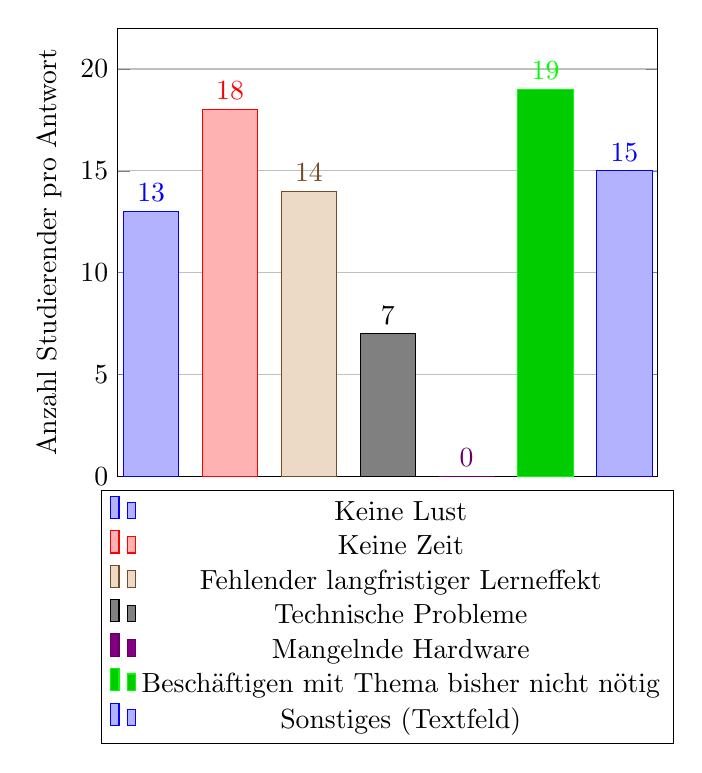
\begin{tikzpicture}
    \begin{axis}[
    	x tick label style={
    		/pgf/number format/1000 sep=},
    	ylabel=Anzahl Studierender pro Antwort,
    	enlarge x limits=2,
        ymax=22,
        ymin=0,
    	legend style={at={(0.5,-0.03)},
        anchor=north,legend columns=1},
        ybar,
        bar width=20pt,
        xticklabels={},
        xtick=\empty,
        nodes near coords,
        grid=major,
    ]
    \addplot coordinates {(1,13)};
    \addplot coordinates {(2,18)};
    \addplot coordinates {(3,14)};
    \addplot coordinates {(4,7)};
    \addplot coordinates {(5,0)};
    \addplot coordinates {(6,19)};
    \addplot coordinates {(7,15)};
    
    \legend{Keine Lust, Keine Zeit, Fehlender langfristiger Lerneffekt, Technische Probleme, Mangelnde Hardware, Beschäftigen mit Thema bisher nicht nötig, Sonstiges (Textfeld)}
    \end{axis}
\end{tikzpicture}
    \caption{Grafische Darstellung der Ergebnisse zur Frage: Mögliche Gründe für Wissensmängel im Bereich}
\end{figure}

Generell bewerteten viele Studierende, trotz dessen, dass viele dieser Git bereits im Studium verwendet hatten, ihre Kenntnisse eher mittelmäßig bis niedrig.

\begin{figure}[h!]
    \centering
    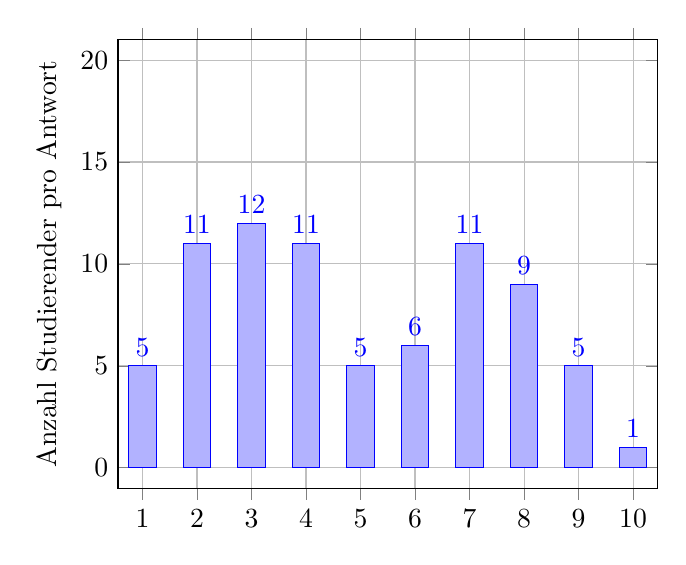
\begin{tikzpicture}
    \begin{axis}[
    	x tick label style={
    		/pgf/number format/1000 sep=},
    	ylabel=Anzahl Studierender pro Antwort,
    	enlargelimits=0.05,
        ymax=20,
        ymin=0,
    	ybar,
        xtick=data,
        xticklabels={1,2,3,4,5,6,7,8,9,10},
        grid=major,
        nodes near coords,
    ]
    \addplot 
    	coordinates {(1,5) (2,11)
    		  (3,12) (4,11) (5,5) (6,6) 
            (7,11) (8,9) (9,5) (10,1)};
    \end{axis}
\end{tikzpicture}
    \caption{Grafische Darstellung der Ergebnisse zur Frage: Wissen von Git}
\end{figure}

Die wichtigste Frage, die mit der Umfrage analysiert werden sollte, ist jedoch die zum Interesse des Systems. 
Durch die Ergebnisse hat sich herausgestellt, dass die Mehrheit der Befragten generell ein Interesse an einem Lernsystem zum Thema Git und GitHub hätte.

\begin{figure}[h!]
    \centering
    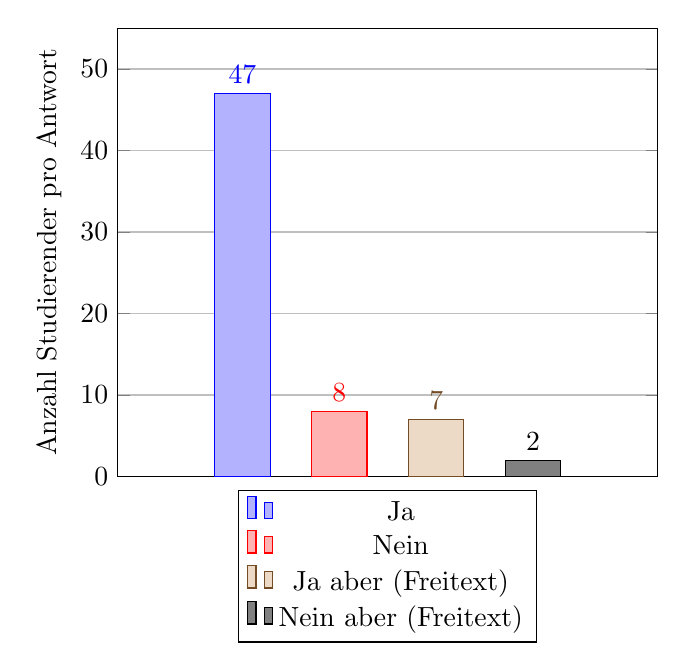
\begin{tikzpicture}
    \begin{axis}[
        x tick label style={
    		/pgf/number format/1000 sep=},
    	ylabel=Anzahl Studierender pro Antwort,
    	enlarge x limits=2,
        ymax=55,
        ymin=0,
    	legend style={at={(0.5,-0.03)},
        anchor=north,legend columns=1},
        ybar,
        bar width=20pt,
        xticklabels={},
        xtick=\empty,
        nodes near coords,
        grid=major,
    ]
    \addplot coordinates {(1,47)};
    \addplot coordinates {(2,8)};
    \addplot coordinates {(3,7)};
    \addplot coordinates {(4,2)};
    
    \legend{Ja, Nein, Ja aber (Freitext), Nein aber (Freitext)}
    \end{axis}
\end{tikzpicture}
    \caption{Grafische Darstellung der Ergebnisse zur Frage: Interessen an einem Lernsystem}
\end{figure}

Zudem ergab sich, dass tiefergehende Lerninhalte generell als wichtiger eingestuft wurden, als ein interessantes Setting mit ansprechendem Humor zu haben.
Im Kontext des Projektes hatte dies zunächst wenig Einwirkung, da der Prototyp um das Konzept der Koch-Analogie strukturiert wurde.

\begin{figure}[h!]
    \centering
    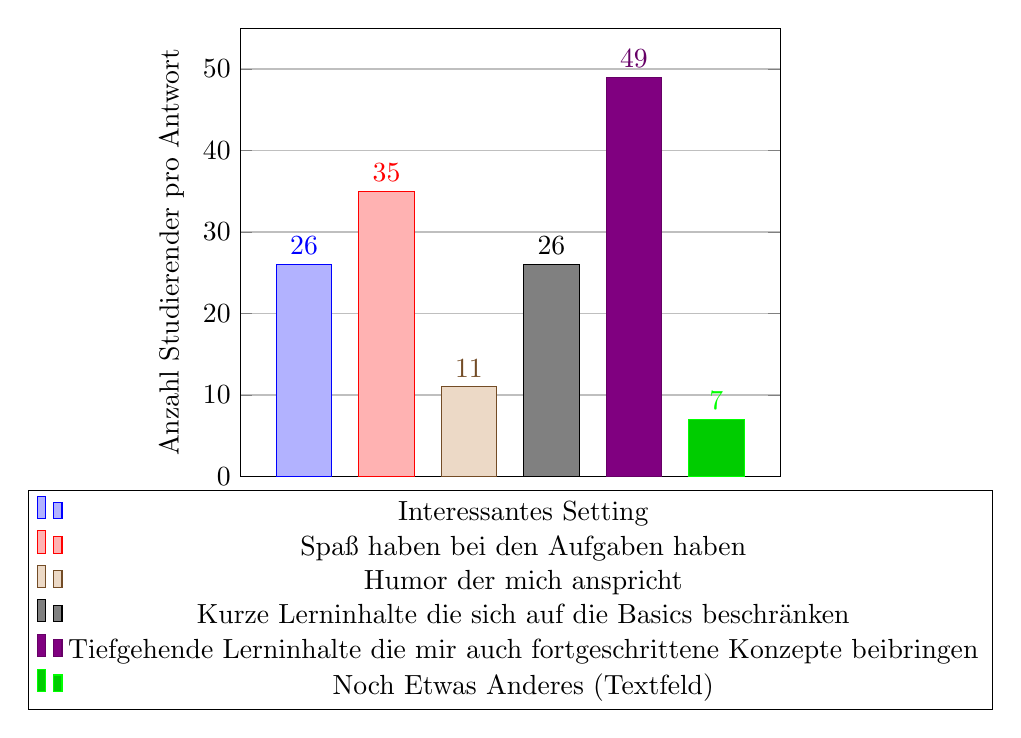
\begin{tikzpicture}
    \begin{axis}[
        x tick label style={
    		/pgf/number format/1000 sep=},
    	ylabel=Anzahl Studierender pro Antwort,
    	enlarge x limits=2,
        ymax=55,
        ymin=0,
    	legend style={at={(0.5,-0.03)},
        anchor=north,legend columns=1},
        ybar,
        bar width=20pt,
        xticklabels={},
        xtick=\empty,
        nodes near coords,
        grid=major,
    ]
    \addplot coordinates {(1,26)};
    \addplot coordinates {(2,35)};
    \addplot coordinates {(3,11)};
    \addplot coordinates {(4,26)};
    \addplot coordinates {(5,49)};
    \addplot coordinates {(6,7)};
    
    \legend{Interessantes Setting, Spaß haben bei den Aufgaben haben, Humor der mich anspricht, Kurze Lerninhalte die sich auf die Basics beschränken, Tiefgehende Lerninhalte die mir auch fortgeschrittene Konzepte beibringen, Noch Etwas Anderes (Textfeld)}
    \end{axis}
    \end{tikzpicture}
    \caption{Grafische Darstellung der Ergebnisse zur Frage: Wünsche an einem Lernsystem}
\end{figure}

Nähere Details zu den Antworten in den Freitextfeldern, sowie die restlichen Inhalte der Umfrageergebnisse befinden sich im Anhang des Projektberichtes.

\chapter{Lösungsansatz}
\label{chap:Textsatz}
Mithilfe der Informationen aus der Problemfeldanalyse wurde eine mögliche Lösung für das Problem entwickelt. 
Im Rahmen des Praxisprojektes sollte so ein Lernsystem für Git und GitHub entwickelt werden, in dem Studierende 
sich selbst Wissen aneignen können, und dieses auch direkt praktisch anwenden, um den Lerneffekt zu verbessern.
\par
Die Frage, wie Gestaltungen eines Systems beim Lernen helfen kann, wurde bereits in den 1990er Jahren von verschiedensten
Forschern untersucht. 
Unter anderem wurden hierbei von Thomas W. Malone Untersuchungen zum Zusammenhang von Computerspielen
und Motivation untersucht.~\cite{malone:tex}
Das oberste Ziel bei der Gestaltung eines Systems bleibt hierbei, dass Nutzende das System nicht aus Zwang nutzen,
sondern aus eigener intrinsischer Motivation.

\par
Dass Spiele beim Lernen von Inhalten ebenfalls effektiver sind, als herkömmliche Materialien, wurde ebenfalls bereits
viel im Kontext des Feldes Gamification untersucht.

\par
Mit dem Lernsystem für Git soll das Wissen daher ebenfalls mittels einer Art Spiel vermittelt werden, in dem die 
Konzepte um Git in eine leichter verständliche Analogie verpackt werden.

\section{Hauptziele des Systems}

Um herauszuarbeiten, was das System leisten muss, wurden zunächst die Phasen der Nutzung ausgearbeitet.
Beispielsweise sollen diese sein, die Motivation, das System zu nutzen, das Verhalten beim Nutzen des Systems,
und anschließend den Lerneffekt, der nachträglich gewonnen werden kann.

Potenzielle Konfliktpunkte des Systems bestehen darin, dass Studierende möglicherweise gar nicht erst zur Nutzung des Systems 
motiviert sind oder im Verlauf der Nutzung feststellen, dass sie Verständnisschwierigkeiten haben, was zu einem 
Abbruch der Nutzung aus Frustration führen könnte.
Daher soll sichergestellt werden, dass Studierende sich mit den Inhalten auseinandersetzen möchten,
andererseits allerdings auch, dass sie die Inhalte verstehen.

\begin{description}
    \item[Motivation zur Nutzung]: Studierende müssen sich grundsätzlich mit dem System auseinandersetzen wollen.
    \item[Nutzung allgemein]: Das System muss einfach gestaltet werden, um Frustration bei der Nutzung zu vermeiden. Im schlimmsten Fall führen Konflikte zum Abbrechen der Nutzung des Systems.
    \item[Lerneffekt]: Damit Studierende eine positive Meinung auf das System behalten und möglicherweise zu diesem zurückkehren oder es weiterempfehlen möchten, muss ein langfristiger Lerneffekt entstehen. Das System sollte zudem ein konsistentes Ende haben, das Nutzende gedanklich mit der Geschichte abschließen lassen.
\end{description}

\par

Weiterhin wurde sich mit den nötigen Hauptfunktionalitäten des Systems auf funktioneller Ebene auseinandergesetzt.
Hierbei wurden Fragen gestellt wie ``Was braucht das System, um erfolgreich zu sein?'', sowie 
``Wie kann die Zielgruppe effektiv angesprochen werden?''.
\par
Es wurden drei Schlüsselpunkte ausgearbeitet.
\begin{description}
    \item[Motivation zum Selbstlernen]: Damit das System Erfolg hat, müssen Studierende das System gerne benutzen. Dazu sollten Frustrationspunkte wie zu schwierige Aufgaben ohne Hilfestellungen oder verwirrende Bedienung vermieden werden.
    \item[Gesammeltes Wissen]: Das System sollte im Idealfall nicht nur zum Lernen der Services dienen, sondern auch als eine Art Nachschlagewerk für alle Kommandos und Abläufe, die man zur Nutzung von Git benötigt. Hierbei werden sich auf die Befehle fokussiert, die direkt in der Kommandozeile ausgeführt werden.
    \item[Zielgruppe und Lerntypen ansprechen]: Damit Studierende motiviert werden, das System zu benutzen, sollte dieses nicht nur einfach zu benutzen sein, sondern die Nutzenden auch auf persönlicher Ebene ansprechen. Hierzu wurde eine Analogie entworfen, die es den Studierenden einfacher machen soll, sich mit den Aufgaben zu identifizieren. Das System soll sich nicht so anfühlen, als wenn man Aufgaben erledigen muss, sondern eher wie ein Spiel, das neben einem langfristigen Lerneffekt den Nutzenden auch Spaß bereitet.
\end{description}

\section{Konzept}
Im Lösungsansatzteil wurde zunächst überlegt, wie man das System konzeptionell gestalten könnte. Hierbei wurden die Grundsätze zunächst technologiefrei entworfen. In späteren Überlegungen, insbesondere im Kontext der Proof of Concepts, wurde bereits grundsätzlich überlegt, welche groben Technologien für das System relevant sind.

\subsection{Analogie}
Die Analogie, die im Kontext der Praxisprojekts gewählt wurde, ist die eines Kochs, der mithilfe von Git Befehlen ein Gericht kocht und anschließend an einen Kunden schickt. Hierbei werden alle nötigen Befehle behandelt und in einzelnen Kapiteln aufgeteilt.
Diese Kapitel umfassen in der derzeitigen Version des Systems:

\begin{enumerate}
    \item Tutorial für die Steuerung des Spiels
    \item Git-Commit durchspielen
    \item Git Branches Erstellen und Verwalten
    \item Merge Konflikte verstehen und lösen
\end{enumerate}

Es wurden vor der Implementierung des Systems verschiedene theoretische Implementierungen dieser Analogie aufgestellt.
Beispielweise wurde überlegt, wie man Branches im Kontext eines Restaurants darstellen könnte. Die Umsetzung der Analogie wurde zusammenfassend in einer Liste gegenübergestellt.

\begin{description}
    \item[git clone] Das kopieren eines Repositorys auf die lokale Maschine sollte im System noch relativ nah an der praktischen Anwendung sein, um Verwirrung zu vermeiden. In der visuellen Darstellung werden durch das erste Klonen alle benötigten Zutaten an den Arbeitsplatz geholt.
    \item[git add] Das Hinzufügen einer Datei wurde mithilfe von Zutaten dargestellt. Hierbei sind drei Lebensmittel zur Verfügung gestellt, ein Blatt Salat, eine Tomate und Hackfleisch. Um einen Burger vollständig zusammenzustellen, werden dann alle Zutaten dem Commit oder visuell dem Burger hinzugefügt und dann verpackt.
    \item[git commit] Das ``Verpacken'' eines Commits wird mithilfe des Burgers visualisiert. Sobald eine Bestellung vollständig hinzugefügt wurde, wird diese abgeschlossen.
    \item[git push] Ein Push wird mit dem Abschicken der Bestellung gleichgesetzt.
    \item[\gls{branches}] Verschiedene Branches sind im Kontext des Systems mit Arbeitsplatten gleichgesetzt. Hierbei können mehrere Köche zusammen an einem Arbeitsplatz arbeiten und sich gegenseitig zuvorkommen, oder an unterschiedlichen Arbeitsplatten arbeiten, und später zu der ``Hauptplatte'' zurückkehren.
    \item[\gls{mergeconflicts}] Merge Konflikte können im System durch überschneidende Zutaten dargestellt werden. Beispielsweise bereitet ein Koch einen Burger ohne Zwiebeln zu, ohne das Wissen, dass in einem späteren Push die Bestellung doch noch aktualisiert wurde, und der Burger nun keine Zwiebeln mehr haben soll.
\end{description}

Im Verlauf der Implementierungsphase wurde die Analogie nicht mehr angepasst.

\subsection{Bedienung}
Das Spiel selbst soll von den Nutzenden über eine Art Mini-Konsole bedient werden, um einen starken Praxisbezug zu gewährleisten.
Studierende sollen, wie sie es auch in einer realen Situation tun würden, über die Konsole die richtigen Befehle eingeben.
Im System wird dieser Prozess durch eine Geschichte unterstützt, und es werden viele Hinweise und Erklärungen gegeben, dazu, welche Befehle eingegeben werden sollen. Mehr dazu, wie genau die Funktionsweise dieser Konsole sein soll, lässt sich in \cref{sec:poc_console} finden.

In der Planung wurde zunächst überlegt, eine möglichst realitätsnahe Konsole auf dem Interface zu haben, die realistische Eingaben und Ausgaben entgegennimmt. Später wurde diese Darstellung allerdings vereinfacht.
Es wurde ebenfalls überlegt, eine tatsächliche Anbindung an GitHub zu haben, über die mit der richtigen Eingabe eines Kommandos ein tatsächliches Repository erstellt wird. Diese Idee wurde allerdings wieder verworfen, da sie annimmt, dass jeder Nutzende des Systems bereits ein GitHub Profil besitzt, beziehungsweise dem System die nötigen Berechtigungen zur \gls{api} Anbindung geben möchte. Außerdem würde dieser Ansatz voraussetzen, dass der Nutzende die Aufgaben in der richtigen Reihenfolge abarbeitet.

Letztendlich wurde sich für eine minimalistische Implementierung der Konsole entschieden, die je nach Aufgabe zugeschnittene Feedbacks bei richtigen und falschen Eingaben geben kann.

\par
Wie die Konsole aussehen soll, wurde zunächst in Wireframes skizziert. Mehr zu dem Thema der Gestaltung lässt sich in \cref{sec:wireframes} finden.

\section{Proof of Concepts}
Bevor mit der Implementierung des Systems begonnen wurde, wurde überlegt, welche die wichtigsten Funktionen sind, und welche Risiken diese bergen könnten. Diese Risiken waren unter anderem wichtig, da ohne die Implementierung möglicher Fallbacks ein Versagen des Systems eintreten könnte.
Mehr zu der Implementierung der jeweiligen Proof of Concepts lässt sich in dem Kapitel zur Implementierung finden.

\subsection{Mock Konsole}
\label{sec:poc_console}
\textbf{Beschreibung}
\newline Einer der wichtigsten Funktionen des Systems ist eine Mock Konsole, auf welcher der Nutzende Eingaben tätigen kann. Nach einer Eingabe soll die Konsole oder das Spiel dem Nutzendem Feedback geben, und das Bild in der Mitte des User-Interfaces soll sich verändern.

\textbf{Exit Kriterium}
\begin{itemize}
    \item Eine richtige Eingabe wurde getätigt, und das Bild in der Mitte hat sich geändert. Die Konsole gibt ein positives Feedback aus.
    \item Eine falsche Eingabe wurde getätigt, und das Bild in der Mitte hat sich nicht geändert. Die Konsole gibt ein negatives Feedback aus.
\end{itemize}
\textbf{Fail Kriterium}
\begin{itemize}
    \item Die Konsole reagiert nicht auf Nutzendeneingaben. 
\end{itemize}

\textbf{Fallback}
\newline Der Nutzende kann in den Einstellungen zwischen manuellen Eingaben und Auswahl aus einem Menü von Befehlen wählen. Diese Befehle haben dieselbe Funktionalität, nur dass der Nutzende diese bereits vorher einsehen kann und die nicht komplett selber eingeben muss.
Dieser Fallback könnte ebenfalls nützlich sein, wenn der Nutzende keine Texteingabe zur Verfügung hat oder die Aufgaben zu schwierig findet, und lieber aus einer Auswahl von Lösungen wählen würde.

\subsection{Dialogeingabe}
\label{sec:poc_dialogue}
\textbf{Beschreibung}
Durch Dialog soll der Nutzende in die Story des Systems gezogen werden und sowohl Erklärungen als auch Feedback zu den Eingaben und Aktionen erhalten. Der Nutzende soll auf die Dialogbox klicken können, um die nächste Dialoglinie angezeigt zu bekommen.
\newline 

\textbf{Exit Kriterium}
\begin{itemize}
    \item Drei Beispieldialoglinien wurden erfolgreich durchgespielt, und der Nutzende kann nun eine Eingabe auf der Mock Konsole durchführen.

\end{itemize}

\textbf{Fail Kriterium}
\begin{itemize}
    \item Der Nutzende weiß nicht, wo dieser klicken muss, um den Dialog fortzuschreiten.
    \item Das System reagiert nicht auf Klicken des Nutzenden, und der Dialog wird nicht fortgesetzt.
\end{itemize}

\textbf{Fallback}
\newline Die Dialogbox weist einen Knopf auf, mit dem der Dialog fortgeschritten werden kann. Zusätzlich kann der Nutzende ebenfalls durch Eingaben über die Tastatur den Dialog fortschreiten.

\subsection{PWA Funktionalitäten}
\label{sec:poc_pwa}
\textbf{Beschreibung}
\newline Das System soll Progressive Webapp (PWA) Funktionen aufweisen, um für den Nutzenden möglichst zugänglich zu sein. Hierzu soll eine offline \gls{html} Seite implementiert sein, die eine sehr simple Version der anderen Proof of Concepts aufweist, mit dem Unterschied, dass es einen Hinweis oben darauf gibt, dass die Seite momentan offline betrachtet wird.

\textbf{Exit Kriterium}
\begin{itemize}
    \item Eine PWA kann erfolgreich installiert werden, und eine Offline Version der Seite kann betrachtet werden.
\end{itemize}

\textbf{Fail Kriterium}
\begin{itemize}
    \item PWA Funktionen nicht verfügbar und Seite lädt trotzdem nicht ordentlich.
\end{itemize}

\textbf{Fallback}
\newline Offline-Funktionen nicht verfügbar machen. Nutzende bekommt einen Hinweis darauf, dass dieser bitte eine Verbindung zum Internet herstellen soll.

\section{Wireframes}
\label{sec:wireframes}
Bevor mit der Implementierung des Systems begonnen wurde, wurden mehrere Skizzierungen zur Gestaltung des Systems erstellt.
Einige ältere Skizzierungen des Levelscreen Designs wurden hierbei ausgelassen.

\begin{figure}[h!]
    \centering
    \includegraphics[width=\textwidth]{Wireframes_Level_V1}
    \caption{Wireframes zur Gestaltung der Levelauswahl}
\end{figure}

\begin{figure}[h!]
    \centering
    \includegraphics[width=\textwidth]{Wireframes_Homescreen_V1}
    \caption{Wireframes zur Gestaltung des Hauptmenüs}
\end{figure}

Die ersten Wireframes sollen die generelle Gestaltung der Menüs skizzieren.
Hierbei sollen alle Level in einer Art Bibliothek gesammelt sein. Die Levels sollen in einer beliebigen Reihenfolge gespielt werden können. Außerdem soll es noch einen weiteren Tab geben, um nur auf die Informationsinhalte zuzugreifen. Im Level selber befinden sich diese unter dem Informations-Button.
Durch eine separate Funktion hierbei soll sichergestellt werden, dass Studierende immer einfachen Zugriff auf alle Informationen haben und alle Kommandos mitsamt ihren Erklärungen an einem gesammelten Ort finden.

\begin{figure}[h!]
    \centering
    \includegraphics[width=\textwidth]{Wireframes_Aufgabe_V2}
    \caption{Wireframes zur Gestaltung des Spiele-Interface}
\end{figure}

Oben dargestellte Grafik soll die Planung des Leveldesigns verdeutlichen. Hierbei wurde unter anderem darauf geachtet, dass das User-Interface minimal gehalten wird, um unnötige Verwirrung zu vermeiden.
Über die Konsole sollen Eingaben getätigt werden, die in dem Bild mittig reflektiert werden. Zudem gibt es eine Menüleiste, in welcher der Nutzende gegebenenfalls ein Level überspringen kann, zurück ins Hauptmenü gelangt oder zusätzliche Erklärungen für das aktuelle Thema aufrufen kann.

Es wurden mehrere verschiedene Skizzen für das Interface erstellt. In der Umsetzung wurde letztendlich eine Kombination verwendet. Links sind die Menüpunkte zu finden, rechts an der Seite ist die Mock Konsole für Eingaben. Mittig in der finalen Version sind das Bild zum Szenario sowie die Dialogbox.
\chapter{Implementierung}
\label{chap:implementation}
Für das System wurde ausschließlich ein Frontend entwickelt, dass in sich geschlossen bereits alle Dialoge und Bilder beinhaltet.

Für die Implementierung wurden verschiedenste Web Technologien verwendet, die in dem Abschnitt Technologien näher beleuchtet werden.

\section{Technologien}
\begin{description}
    \item \textbf{CSS und Tailwind} Für das generelle Styling des Frontends wurde im Projekt Tailwind CSS eingesetzt. Dieses Framework erleichtert es, Änderungen schnell und effizient umzusetzen und somit eine möglichst kurze Feedback-Schleife sicherzustellen. In Kombination mit Vite wurden bei Änderungen im Styling der Server direkt neu geladen, was den Entwicklungsprozess um vieles vereinfachte.
    \item \textbf{Typescript} Als Programmiersprache für logische Funktionen wurde TypeScript statt Javascript verwendet, um es einfacher zu machen, Klassen und Interfaces zu erstellen, sowie eine Typsicherheit zu gewährleisten.
    \item \textbf{Vite/Vue/HTML} HTML wurde im Projekt in Verbindung mit Vue.js verwendet. Vite diente zum Erstellen des Grundgerüsts des Vue-Projekts. Anschließend wurde der integrierte Entwicklungsserver von Vite genutzt, um eine möglichst schnelle Feedback-Schleife für visuelle Anpassungen zu ermöglichen.
    \item \textbf{Deno} Deno wurde in diesem Projekt als Alternative zu Node.js verwendet. Dies erfolgte teils aus persönlichem Interesse, um die neue Technologie zu erlernen. Deno wurde als Ersatz für Node.js, da es von den selben Entwicklern stammt, und mehr Features bietet, die mehr Entwicklungsfreiraum für die Zukunft bieten als herkömmliche Laufzeitumgebungen. Zusätzlich bietet es eine Rückwärtskompatibilität mit Node.js, die alle alten Bibliotheken unterstützt.
    \item \textbf{PWA Funktionalitäten} Zu Beginn des Projektes wurde überlegt, wie man das System möglichst zugänglich machen kann. Zunächst wurde in Erwägung gezogen, das System als Desktop Applikation zu implementieren. Hierzu wäre das Framework Electron verwendet worden. Hierbei könnten alle bisher erwähnten Frameworks wie gewohnt verwendet werden. In mehreren Beratungsgesprächen hatte sich allerdings herausgestellt, dass es sinnvoller wäre, eine Webapp zu entwickeln, die unabhängig vom System des Nutzenden funktioniert, und zudem Offline Funktionen aufweist. Es wurde sich daher entschieden, das System als Web-Applikation mit progressive Webapp (PWA) Funktionen zu implementieren. Grund hierfür war unter anderem, dass die Applikation möglichst unabhängig funktionieren soll und auch die Möglichkeit bieten soll, heruntergeladen zu werden. Studierende können hierbei eine lokale Version des Systems auf ihren Geräten haben.
\end{description}

\section{Implementierung der Proof of Concepts}
Im folgenden Abschnitt werden alle Proof of Concepts noch einmal reflektiert betrachtet. Hierbei wird sich auf die ausformulierten Proof of Concepts aus \cref{chap:Textsatz} bezogen.
\subsection{Mock Konsole} \footnote{\url{https://github.com/AnoukMartinez/martinez-pp-ss-2024/blob/main/src/components/Console.vue}}
Die Mock Konsole wurde anhand einer Vue Komponente implementiert, die an bestimmten Stellen im Dialog automatisch aktiviert und deaktiviert wird. Bei Eingaben wird ein Feedback innerhalb der Konsole ausgegeben, welches zu der Aufgabe passt.

Der Fallback für auswählbare Optionen wurde im Rahmen des Praxisprojektes nicht erstellt. Der zeitliche Rahmen war ungenügend. Außerdem wurden letztendlich andere Features als wichtiger eingestuft.

\subsection{Dialog}
Der Dialog wurde ebenfalls in einer eigenen Vue Komponente umgesetzt. \footnote{\url{https://github.com/AnoukMartinez/martinez-pp-ss-2024/blob/main/src/components/DialogueBox.vue}}
Wenn keine Eingabe benötigt wird, kann der Nutzende des Systems auf die Dialog-Box klicken, um die nächste Zeile zu sehen.
Es wurde zudem entschieden, einige Wörter hervorzuheben, die besonders wichtig sind, oder einen Hinweis auf die kommende Eingabe geben sollen.
Wenn keine Eingabe nötig ist, wird dem Nutzendem ebenfalls ein Hinweis gegeben.

\subsection{PWA Funktionalitäten}
Die PWA Funktionen wurde zu Beginn der Implementierung eingerichtet, und funktionieren online. Die Anwendung ist herunterladbar, benötigt allerdings trotzdem eine Verbindung zum Server.
In der momentanen Version der Applikation gibt es daher keine Offline Funktionalitäten.

\chapter{Fazit und Reflexion}
Abschließend werden noch einmal alle Teile des Projekts reflektiert betrachtet. Zudem werden mögliche zukünftige Funktionen des Projekts betrachtet.

\section{Schwierigkeiten bei der Implementierung}
Eine der größten Herausforderungen bei der Umsetzung des Systems war die Organisation der Vue-Komponenten. Zwar war im Vorfeld geplant, dass beispielsweise bei Nutzendeneingaben ein entsprechendes Feedback generiert werden soll, jedoch wurde die Kommunikation zwischen den Komponenten nicht detailliert genug durchdacht. Stattdessen erfolgte die Implementierung situationsbedingt, abhängig von den jeweils benötigten Funktionalitäten.

Dies lag teilweise daran, dass sich die Funktionsweise von Vue generell erst während der Projektarbeit parallel beigebracht wurde. 
So war es intransparent, wie die Komponenten strukturiert werden sollten.

Dies führte zu einem anfänglich komplexen und unübersichtlichen Einsatz von Vue-Emits, der im weiteren Verlauf der Entwicklung schrittweise reduziert und vereinfacht werden musste.

\subsection{Analogie}
Was zudem größtenteils zu Schwierigkeiten führte, war vor allem der Einsatz einer Analogie zum Erklären der Sachverhalte. Besonders herausfordernd war, immer Äquivalente zu den Themen zu finden, die mit der Analogie erklärbar sind.
Beispielsweise war es sehr schwierig, einen sinnvollen Vergleich für das Klonen und Pullen eines Repository zu finden.

Aus der Umfrage der Studierenden ergab sich, dass die Inhalte eine höhere Priorität einnehmen als das Setting und die Geschichte, die eventuell mit dem System kommt.
Vor allem im Hinblick auf die Umfrageergebnisse lässt sich daher rückblickend sagen, dass die Verwendung einer Analogie im Kontext eines Lernsystems für Git eher ungeeignet ist.
Im Falle der weiteren Entwicklung des Systems sollte die Analogie durch simple, praxisbezogene Visualisierungen ersetzt werden.

Das größte Risiko bei der Verwendung einer Analogie ist hierbei Verwirrung unter den Nutzenden. 
Um nicht den gesamten Fortschritt rückgängig zu machen, der im Rahmen des Projektes geleistet wurde, könnte dem Nutzenden eine Wahl gegeben werden, zwischen einem \gls{storymode} und einem Modus, der sich nur auf die Lerninhalte fokussiert.

\section{Zukünftige Ergänzungen}
Insgesamt lässt sich sagen, dass das Projekt momentan noch nicht in einem Zustand ist, in dem das System praktisch anwendbar wäre.
Für die Fertigstellung eines minimal realisierbaren Systems fehlen noch folgende Aspekte:

\begin{description}
    \item[Rückmeldungen] Um das System benutzendenfreundlich und effizient zu gestalten, ist es notwendig, Rückmeldungen von Testnutzenden einzuholen. Auf Basis dieser Rückmeldungen muss das System detailliert angepasst werden, um eine frustrationsfreie Lernerfahrung zu gewährleisten.
    \item[Erklärungen] Um einen besseren Lerneffekt zu gewährleisten, wurde ein Infoknopf in der Seitenleiste eingebaut, der für jedes Kapitel zusätzliche Erklärungen bereitstellen soll. Diese Erklärungen sind allerdings nur teilweise geschrieben worden, und erfordern noch einer inhaltlichen Erweiterung.
    \item[Weitere Kapitel] Für die inhaltliche Vervollständigung des Systems fehlt ein Kapitel zum Thema Merge-Konflikte. Dieses wurde im Rahmen des Projekts nicht umgesetzt, da es den zeitlichen Umfang überschritten hätte. Zusätzlich wäre ein Mock-Editor zu integrieren, in dem Nutzende Merge-Konflikte simulieren können. Hierbei muss die Eingabe semantisch geprüft werden.
    \item[Verständlicheres Feedback] Eine sinnvolle Ergänzung des Systems wären Ausgaben in der Konsole, die eine echte Ausgabe in der Git Bash simulieren.
\end{description}

Zudem könnten folgende optionale Funktionen noch zusätzlich implementiert werden. Diese sind allerdings nicht zwingender Weise für die Fertigstellung des Projektes benötigt.

\begin{description}
    \item[Fallback für Konsoleneingaben] Wie in den Proof of Concepts erwähnt, war initial eine Alternative für Texteingaben geplant, in welcher der Nutzende aus einer Auswahl an Kommandos durch Klicken wählen kann. Dann können Nutzende des Systems in den Einstellungen den Modus auswählen, den sie präferieren.
    \item[Offline-Funktionen] Zuletzt sollten dem System Offline-Funktionen im Kontext der PWA-Funktion gegeben werden, um möglichst zugänglich für alle Studierenden zu sein. 
\end{description}
%
\printbibliography
%
\appendix
\addchap{Anhang}
\KOMAoptions{open=any}
\newline

Im Rahmen der Projektarbeit wurde eine Umfrage unter Studierenden der Fakultät 10 durchgeführt. 
Teilnehmende sollten hierbei verschiedene Fragen zum Thema Git, GitHub und ihrer Demografik beantworten. 
Im folgendem Abschnitt sind die vollständigen Ergebnisse dieser Umfrage zu finden.
\par
Bei einigen Fragen wurden Freitextfelder zur Verfügung gestellt. 
Die Ergebnisse dieser Felder sind gesondert in Listen direkt unter den grafischen Darstellungen zu finden. \newline 
Zudem anzumerken ist, dass zwei Unfragen parallel durchgeführt wurden, einmal in deutscher Sprache, und einmal in englischer Sprache verfasst. 
Diese Maßnahme wurde getätigt, um die Umfrage möglichst zugänglich zu machen, und um möglichst viele diverse Antworten zu erhalten. 
Alle im Abschnitt dargestellten Ergebnisse sind eine Kombination beider Ergebnisse. Die Fragestellungen wurden hierbei identisch formuliert. 
Alle Antworten wurden am letzten Stand, dem 08.10.2024 um 15:35 abgerufen.

\newpage
{\LARGE \textbf{Demografik}}
\newline

% Studiengang
\begin{figure}[h!]
    \centering
    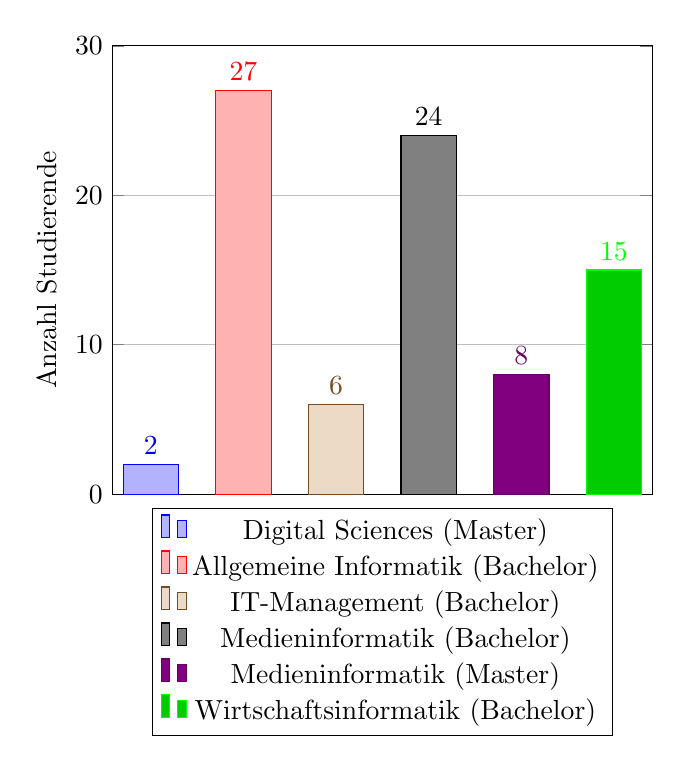
\begin{tikzpicture}
    \begin{axis}[
            x tick label style={
                /pgf/number format/1000 sep=},
            ylabel=Anzahl Studierende,
            enlarge x limits=1.2,
            ymax=30,
            ymin=0,
            legend style={at={(0.5,-0.03)},
            anchor=north,legend columns=1},
            ybar,
            bar width=20pt,
            xticklabels={},
            xtick=\empty,
            nodes near coords,
            grid=major,
        ]
        
        \addplot coordinates {(1,2)}; % DS
        \addplot coordinates {(2,27)}; % AI
        \addplot coordinates {(3,6)}; % ITM
        \addplot coordinates {(4,24)}; % MIB
        \addplot coordinates {(5,8)}; % MIM
        \addplot coordinates {(6,15)}; % WI
        
        \legend{Digital Sciences (Master), Allgemeine Informatik (Bachelor), IT-Management (Bachelor), Medieninformatik (Bachelor), Medieninformatik (Master), Wirtschaftsinformatik (Bachelor)}
    \end{axis}
\end{tikzpicture}
    \caption{Grafische Darstellung der Ergebnisse zur Frage: Studiengänge der Teilnehmer}
\end{figure}

% Semester
\begin{figure}[h!]
    \centering
    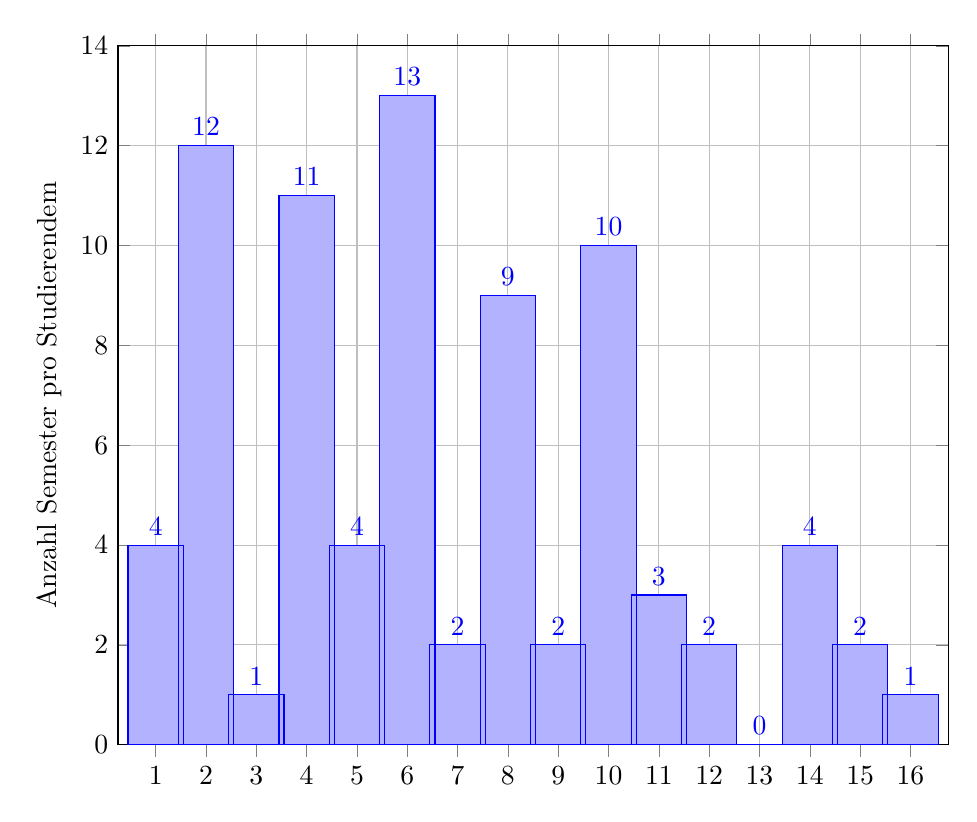
\begin{tikzpicture}
    \begin{axis}[
        x tick label style={
            /pgf/number format/1000 sep=},
        ylabel=Anzahl Semester pro Studierendem,
        enlarge x limits=0.05,
        ymax=14,
        ymin=0,
        ybar,
        bar width=20pt,
        xtick=data,
        xticklabels={1,2,3,4,5,6,7,8,9,10,11,12,13,14,15,16}, 
        width=\linewidth,
        nodes near coords,
        grid=major,
    ]
    
    \addplot coordinates {(1,4) (2,12) (3,1) (4,11) (5,4) (6,13) (7,2) (8,9) (9,2)
    (10,10) (11,3) (12,2) (13,0) (14,4) (15,2) (16,1)};
    \end{axis}
\end{tikzpicture}
    \caption{Grafische Darstellung der Ergebnisse zur Frage: Semester der Teilnehmer}
\end{figure}

% Betriebssysteme
\begin{figure}[h!]
    \centering
    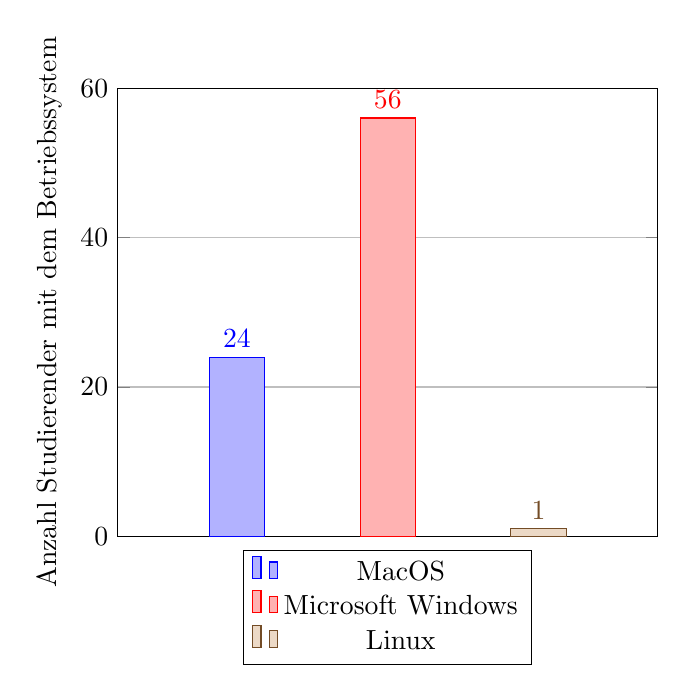
\begin{tikzpicture}
    \begin{axis}[
        x tick label style={
            /pgf/number format/1000 sep=},
        ylabel=Anzahl Studierender mit dem Betriebssystem,
        enlarge x limits=1,
        ymax=60,
        ymin=0,
        legend style={at={(0.5,-0.03)},
        anchor=north,legend columns=1},
        ybar,
        bar width=20pt,
        xtick=\empty,
        xticklabels={},
        nodes near coords,
        grid=major,
    ]
    
    \addplot coordinates {(1,24)}; % macOS
    \addplot coordinates {(2,56)}; % Windows
    \addplot coordinates {(3,1)}; % Linux
    
    \legend{MacOS, Microsoft Windows, Linux}
    \end{axis}
\end{tikzpicture}
    \caption{Grafische Darstellung der Ergebnisse zur Frage: Betriebssysteme der Teilnehmer}
\end{figure}

% Unterschied Git und Github
\begin{figure}[h!]
    \centering
    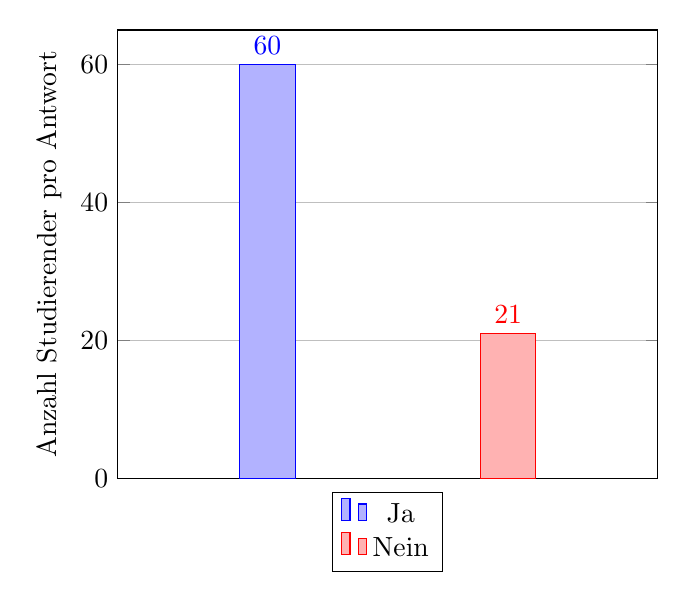
\begin{tikzpicture}
    \begin{axis}[
        x tick label style={
            /pgf/number format/1000 sep=},
        ylabel=Anzahl Studierender pro Antwort,
        enlarge x limits=1,
        ymax=65,
        ymin=0,
        legend style={at={(0.5,-0.03)},
        anchor=north,legend columns=1},
        ybar,
        bar width=20pt,
        xtick=\empty,
        xticklabels={},
        nodes near coords,
        grid=major,
    ]
    
    \addplot coordinates {(1,60)}; % Ja
    \addplot coordinates {(2,21)}; % Nein
    
    \legend{Ja, Nein}
    \end{axis}
\end{tikzpicture}
    \caption{Grafische Darstellung der Ergebnisse zur Frage: ``Ich kenne den Unterschied zwischen Git und Code Hosting Plattformen wie GitHub.''}
\end{figure}

\newpage
{\LARGE \textbf{Git und Github Erfahrungen}}

Im Abschnitt der Umfrage zu Erfahrungen sollte sichergestellt werden, dass die Befragten sich bereits mit Git auseinandersetzen mussten.
Zudem sollte erforscht werden, in welchem Zusammenhang Git verwendet wurde, und welche Schnittstellen zu Nutzung verwendet wurden.

% Hat bereits an Kursen teilgenommen, in denen Git/Github verwendet wurde
\begin{figure}[h!]
    \centering
    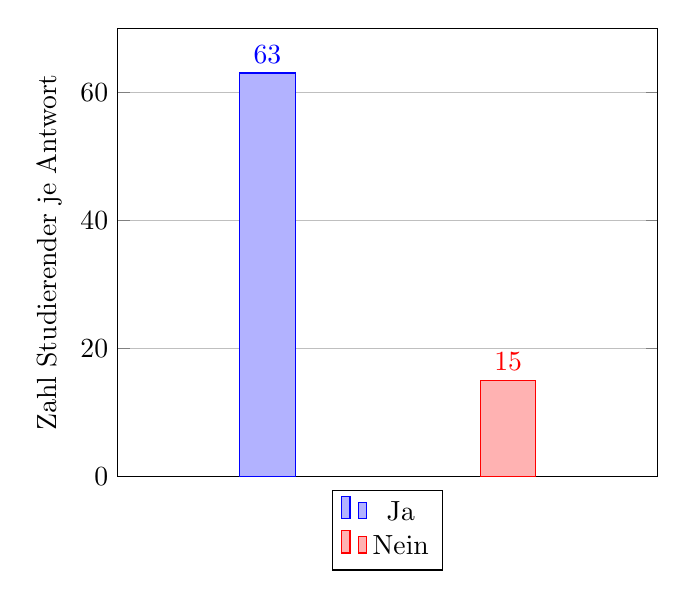
\begin{tikzpicture}
    \begin{axis}[
        x tick label style={
            /pgf/number format/1000 sep=},
        ylabel=Zahl Studierender je Antwort,
        enlarge x limits=1,
        ymax=70,
        ymin=0,
        legend style={at={(0.5,-0.03)},
        anchor=north,legend columns=1},
        ybar,
        bar width=20pt,
        xtick=\empty,
        xticklabels={},
        nodes near coords,
        grid=major,
    ]
    
    \addplot coordinates {(1,63)}; % Ja
    \addplot coordinates {(2,15)}; % Nein
    
    \legend{Ja, Nein}
    \end{axis}
\end{tikzpicture}
    \caption{Grafische Darstellung der Ergebnisse zur Frage: ``Ich habe bereits im Rahmen meines Studiums an ein oder mehreren Kursen teilgenommen, in denen die Nutzung von Git oder Services wie GitHub erforderlich war.''}
\end{figure}

% Git/Github an der TH
\begin{figure}[h!]
    \centering
    \input{tikz/survey/figAnTH}
    \caption{Grafische Darstellung der Ergebnisse zur Frage: ``Ich habe bereits Git oder Services wie GitHub im Kontext meiner Projekte der Hochschule verwendet.''}
\end{figure}

% Git/Github für Arbeit
\begin{figure}[h!]
    \centering
    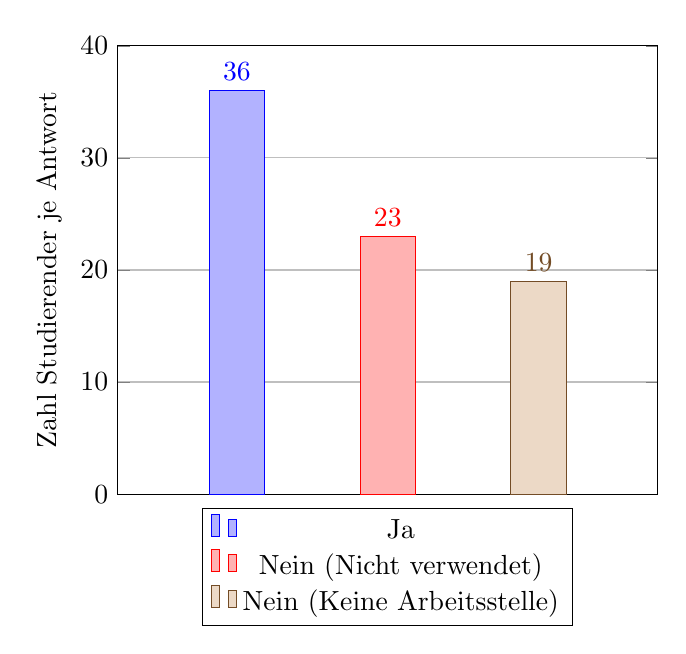
\begin{tikzpicture}
    \begin{axis}[
        x tick label style={
            /pgf/number format/1000 sep=},
        ylabel=Zahl Studierender je Antwort,
        enlarge x limits=1,
        ymax=40,
        ymin=0,
        legend style={at={(0.5,-0.03)},
        anchor=north,legend columns=1},
        ybar,
        bar width=20pt,
        xtick=\empty,
        xticklabels={},
        nodes near coords,
        grid=major
    ]
    
    \addplot coordinates {(1,36)}; % Ja
    \addplot coordinates {(2,23)}; % Nein
    \addplot coordinates {(3,19)}; % Nein (Keine Arbeit momentan)
    
    \legend{Ja, Nein (Nicht verwendet), Nein (Keine Arbeitsstelle)}
    \end{axis}
\end{tikzpicture}
    \caption{Grafische Darstellung der Ergebnisse zur Frage: ``Ich habe bereits Git oder Services wie GitHub im Rahmen meiner Arbeit verwendet.''}
\end{figure}

% Git/Github für private Projekte
\begin{figure}[h!]
    \centering
    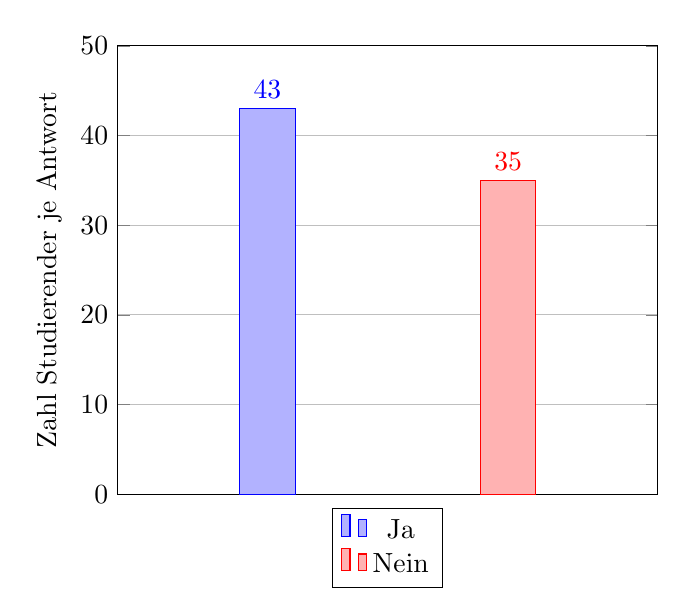
\begin{tikzpicture}
    \begin{axis}[
        x tick label style={
            /pgf/number format/1000 sep=},
        ylabel=Zahl Studierender je Antwort,
        enlarge x limits=1,
        ymax=50,
        ymin=0,
        legend style={at={(0.5,-0.03)},
        anchor=north,legend columns=1},
        ybar,
        bar width=20pt,
        xtick=\empty,
        xticklabels={},
        nodes near coords,
        grid=major,
    ]
    
    \addplot coordinates {(1,43)};
    \addplot coordinates {(2,35)};
    
    \legend{Ja, Nein}
    \end{axis}
\end{tikzpicture}
    \caption{Grafische Darstellung der Ergebnisse zur Frage: ``Ich habe bereits Git oder Services wie GitHub im Kontext meiner persönlichen privaten Projekte verwendet.''}
\end{figure}

% GUI Client
\begin{figure}[h!]
    \centering
    \input{tikz/survey/figGUI}
    \caption{Grafische Darstellung der Ergebnisse zur Frage: ``Ich habe schon einmal einen GitHub GUI Client verwendet.''}
\end{figure}

% Grafisches Interface
\begin{figure}[h!]
    \centering
    \input{tikz/survey/figGrafischesInterface}
    \caption{Grafische Darstellung der Ergebnisse zur Frage: ``Ich habe schon einmal GitHub über das integrierte grafische Interface einer IDE verwendet.''}
\end{figure}

% Git über Kommandozeile
\begin{figure}[h!]
    \centering
    \begin{tikzpicture}
    \begin{axis}[
        x tick label style={
            /pgf/number format/1000 sep=},
        ylabel=Zahl Studierender je Antwort,
        enlarge x limits=1,
        ymax=65,
        ymin=0,
        legend style={at={(0.5,-0.03)},
        anchor=north,legend columns=1},
        ybar,
        bar width=20pt,
        xtick=\linewidth,
        xticklabels={},
        nodes near coords,
        grid=major,
    ]
    
    \addplot coordinates {(1,61)}; % Ja
    \addplot coordinates {(2,16)}; % Nein
    
    \legend{Ja, Nein}
    \end{axis}
\end{tikzpicture}
    \caption{Grafische Darstellung der Ergebnisse zur Frage: ``Ich habe bereits Git über die Kommandozeile verwendet.''}
\end{figure}

\newpage
{\LARGE \textbf{Selbsteinschätzung der Teilnehmenden}}

Im dritten Teil der Umfrage wurde Teilnehmenden eine Möglichkeit gegebene, ihre eigenen Kompetenzen einzuschätzen und zu bewerten.
Hierbei wurden verschiedenste Aussagen getätigt, dessen Zutreffen im Anschluss auf einer Skala von Eins bis Zehn bewertet wurden.

Dabei wurde der folgende Info Text mit den ungefähren Vergleichswerten beigefügt. Hierbei soll eine 1 auf der Skala etwa vergleichbar sein mit der Aussage ``Ich habe noch nie von dem Service/Tool gehört''. 
Eine 10 hingegen soll auf der Skala vergleichbar sein mit der Aussage ``Ich habe den Service/das Tool vollkommen verstanden und kenne ein paar fortgeschrittene Konzepte''.
Fortgeschrittene Konzepte sollen hier beispielsweise Branches für Git sein, oder generelle Code Review Funktionen für GitHub. Diese Vergleiche wurdem im Kontext der Umfrage in der Fragestellung spezifiziert.

% Wissen Git
\begin{figure}[h!]
    \centering
    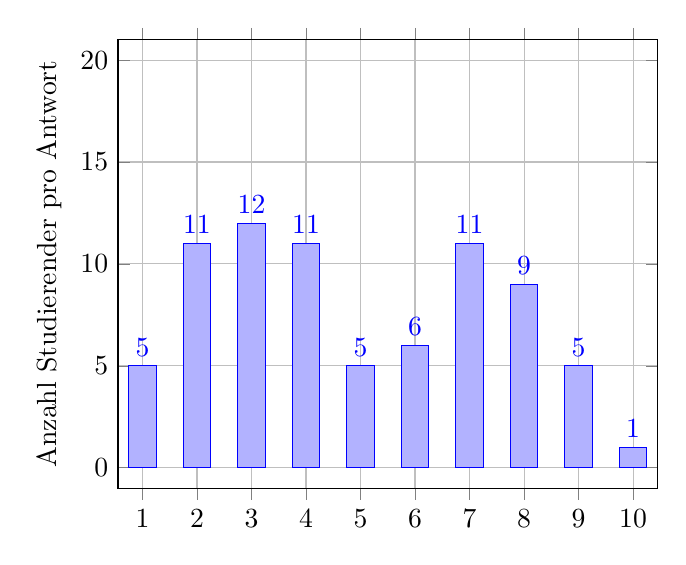
\begin{tikzpicture}
    \begin{axis}[
    	x tick label style={
    		/pgf/number format/1000 sep=},
    	ylabel=Anzahl Studierender pro Antwort,
    	enlargelimits=0.05,
        ymax=20,
        ymin=0,
    	ybar,
        xtick=data,
        xticklabels={1,2,3,4,5,6,7,8,9,10},
        grid=major,
        nodes near coords,
    ]
    \addplot 
    	coordinates {(1,5) (2,11)
    		  (3,12) (4,11) (5,5) (6,6) 
            (7,11) (8,9) (9,5) (10,1)};
    \end{axis}
\end{tikzpicture}
    \caption{Grafische Darstellung der Ergebnisse zur Frage: Wissen von Git}
\end{figure}

% Wissen Github
\begin{figure}[h!]
    \centering
    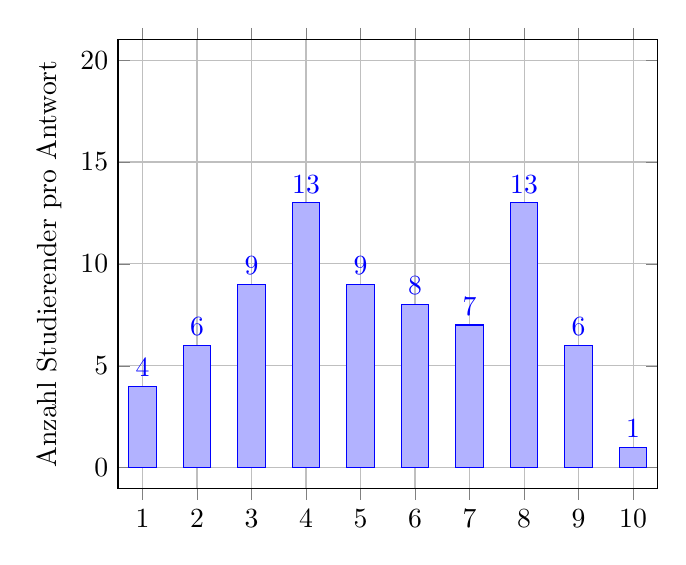
\begin{tikzpicture}
    \begin{axis}[
    	x tick label style={
    		/pgf/number format/1000 sep=},
    	ylabel=Anzahl Studierender pro Antwort,
    	enlargelimits=0.05,
        ymax=20,
        ymin=0,
    	ybar,
        xtick=data,
        xticklabels={1,2,3,4,5,6,7,8,9,10},
        grid=major,
        nodes near coords,
    ]
    \addplot 
    	coordinates {(1,4) (2,6)
    		  (3,9) (4,13) (5,9) (6,8) 
            (7,7) (8,13) (9,6) (10,1)};
    \end{axis}
\end{tikzpicture}
    \caption{Grafische Darstellung der Ergebnisse zur Frage: Wissen von GitHub}
\end{figure}

% Wissen anderer Services
\begin{figure}[h!]
    \centering
    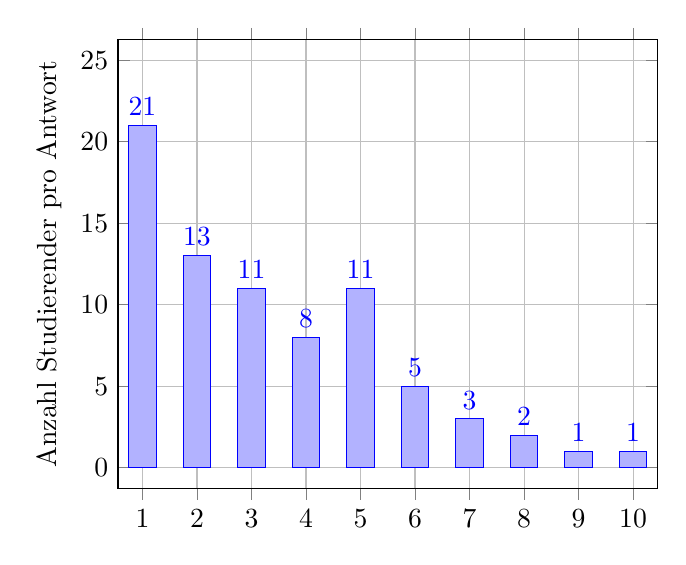
\begin{tikzpicture}
    \begin{axis}[
    	x tick label style={
    		/pgf/number format/1000 sep=},
    	ylabel=Anzahl Studierender pro Antwort,
    	enlargelimits=0.05,
        ymax=25,
        ymin=0,
    	ybar,
        xtick=data,
        xticklabels={1,2,3,4,5,6,7,8,9,10},
        grid=major,
        nodes near coords,
    ]
    \addplot 
    	coordinates {(1,21) (2,13)
    		  (3,11) (4,8) (5,11) (6,5) 
            (7,3) (8,2) (9,1) (10,1)};
    \end{axis}
\end{tikzpicture}
    \caption{Grafische Darstellung der Ergebnisse zur Frage: Wissen von Anderen Services}
\end{figure}

\newpage
{\LARGE \textbf{Interesse an einem Lernsystem}}

Um anhand der Umfrage bestätigen zu können, ob ein Lernsystem wirklich von der Zielgruppe gewünscht wird, wurde die Frage speziell in einem eigenem Teil behandelt.
Hierbei wurde unter anderem gefragt, ob Studierende generell Interesse an einem Lernsystem hätten, sowie was ihnen bei einem solchem System wichtig wäre.

Zunächst wurden die möglichen Wissensmängel in einer Selbsteinschätzung der Studierenden betrachtet. Hierbei wurde ebenfalls die Möglichkeit gegeben, ein Freitextfeld auszuwählen. 
Die gegebenen Antworten sind ebenfalls in diesem Dokument beschrieben, jeweils in einer Auslistung unter der grafischen Darstellung der vorgegebenen Ergebnisse.

% Gründe für Mängel
\begin{figure}[h!]
    \centering
    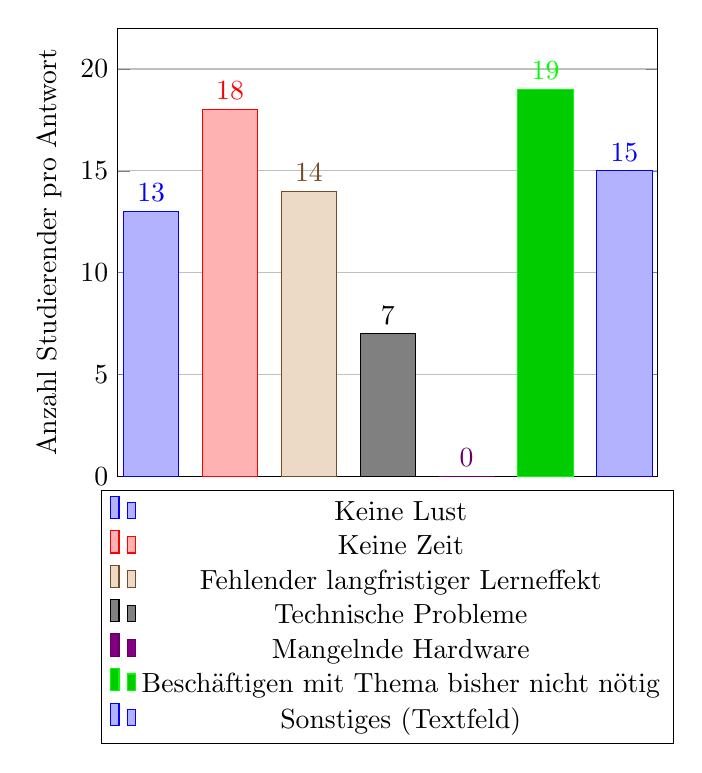
\begin{tikzpicture}
    \begin{axis}[
    	x tick label style={
    		/pgf/number format/1000 sep=},
    	ylabel=Anzahl Studierender pro Antwort,
    	enlarge x limits=2,
        ymax=22,
        ymin=0,
    	legend style={at={(0.5,-0.03)},
        anchor=north,legend columns=1},
        ybar,
        bar width=20pt,
        xticklabels={},
        xtick=\empty,
        nodes near coords,
        grid=major,
    ]
    \addplot coordinates {(1,13)};
    \addplot coordinates {(2,18)};
    \addplot coordinates {(3,14)};
    \addplot coordinates {(4,7)};
    \addplot coordinates {(5,0)};
    \addplot coordinates {(6,19)};
    \addplot coordinates {(7,15)};
    
    \legend{Keine Lust, Keine Zeit, Fehlender langfristiger Lerneffekt, Technische Probleme, Mangelnde Hardware, Beschäftigen mit Thema bisher nicht nötig, Sonstiges (Textfeld)}
    \end{axis}
\end{tikzpicture}
    \caption{Grafische Darstellung der Ergebnisse zur Frage: Mögliche Gründe für Wissensmängel im Bereich}
\end{figure}

Freitext: Sonstige Gründe für Wissensmängel
\begin{itemize}
    \setlength{\itemsep}{-1pt} 
    \item An der Th wurde es nicht richtig erklärt bzw. beigebracht bekommen
    \item Ich weiß wie Git funktioniert, weiß aber auch, dass mein Wissen nicht wirklich über die Basics hinausgeht.
    \item Es besteht keine Notwendigkeit
    \item Keine Erklärungen in den Fächern. Man wird einfach rein geworfen. Hätte mir eine kleine einführung gewünscht
    \item Gute Git/Hub Kenntnisse sind kein muss. Meistens reichen einfache Push/Pull/Clone Aktionen.
    \item Ich musste mich bisher nicht mehr in das Thema einarbeiten. Damit ist gemeint, dass ca. 6 Befehle alle meine Use-Cases bis jetzt abgedeckt haben.
    \item Alles Wissen das ich besitze habe ich aufgrund von erfahrenen Freunden. Den richtigen Umgang oder irgendetwas im Allgemeinen dazu wurde an der TH nie (verständlich) beigebracht sondern immer einfach vorrausgesetzt
    \item Beim selber erlernen bringt man sich aus Zeitgründen nur das nötigste bei, um die Aufgaben erfüllen zu können. Wenn es danach nicht mehr gebraucht wird wird das Gelernte wieder vergessen.
    \item Man geht in der Hochschule quasi nie über das Klonen und Pushen hinaus.
    \item Wozu reines Git wenn es Github gibt
    \item Nur mit minimalen funktionen in bestimtmen kursen. Es wird nie regelmäßig verwendet, sodass ein regelmäßiger kontakt mit git entstanden ist
    \item Wird in den Vorlesung nur kurz vorgestellt und dann soll man alles darüber wissen I guess...
    \item nach einer Zeit wenn man es nicht mehr verwendet, ist das Wissen sehr darüber sehr schwammig. Und die Basis wieder nochmals aufzuholen, ist immer eine sehr hohe Hürde.
    \item Bisher war es nie sonderlich zwingend, daher war die Motivation nicht sonderlich hoch. Und nach dem Benutzen (was selten war), habe ich alles wieder vergessen
    \item nicht oft genug damit gearbeitet.
\end{itemize}

% Wünsche für Lernsystem
\begin{figure}[h!]
    \centering
    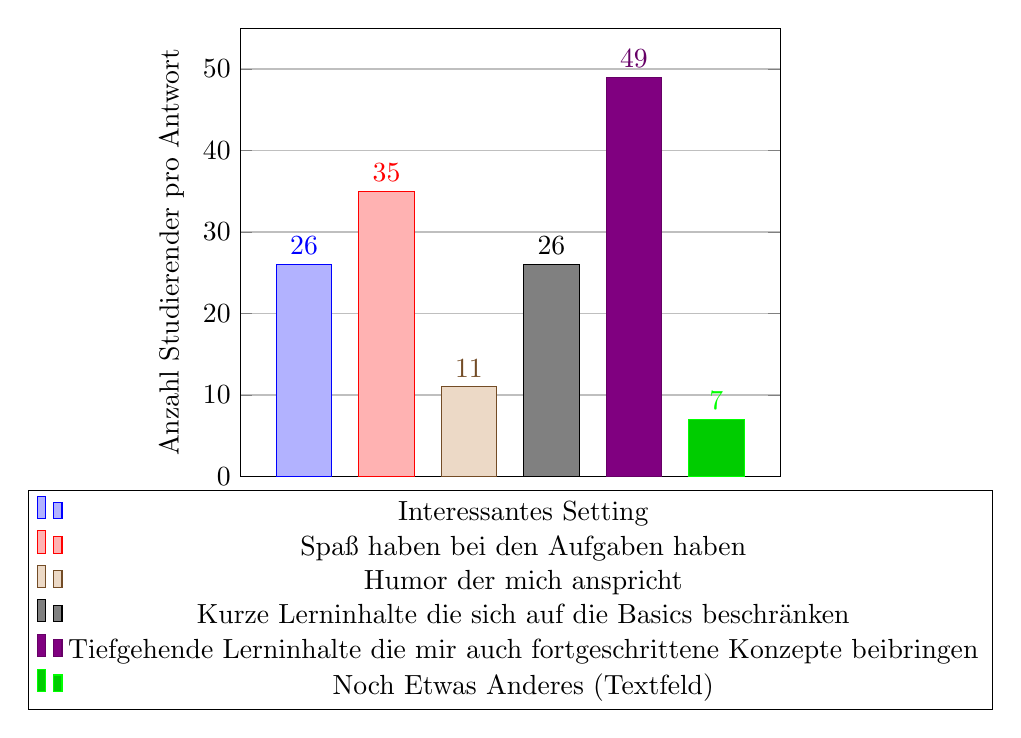
\begin{tikzpicture}
    \begin{axis}[
        x tick label style={
    		/pgf/number format/1000 sep=},
    	ylabel=Anzahl Studierender pro Antwort,
    	enlarge x limits=2,
        ymax=55,
        ymin=0,
    	legend style={at={(0.5,-0.03)},
        anchor=north,legend columns=1},
        ybar,
        bar width=20pt,
        xticklabels={},
        xtick=\empty,
        nodes near coords,
        grid=major,
    ]
    \addplot coordinates {(1,26)};
    \addplot coordinates {(2,35)};
    \addplot coordinates {(3,11)};
    \addplot coordinates {(4,26)};
    \addplot coordinates {(5,49)};
    \addplot coordinates {(6,7)};
    
    \legend{Interessantes Setting, Spaß haben bei den Aufgaben haben, Humor der mich anspricht, Kurze Lerninhalte die sich auf die Basics beschränken, Tiefgehende Lerninhalte die mir auch fortgeschrittene Konzepte beibringen, Noch Etwas Anderes (Textfeld)}
    \end{axis}
    \end{tikzpicture}
    \caption{Grafische Darstellung der Ergebnisse zur Frage: Wünsche an einem Lernsystem}
\end{figure}

Freitext: Sonstige Wünsche für ein Lernsystem
\begin{itemize}
    \setlength{\itemsep}{-1pt} 
    \item simplere gestaltung
    \item Visualisierungen!!
    \item Einen gut verständlichen Einstieg der nicht überfordert und sich auf die Basics beschränkt mit aufbauend schwerer werdenden Lerninhalten
    \item in kleiner abschließbare Module unterteilen, dass es nicht so ein großer Block ist
    \item Active Recall, Spaced Repetition, Interleaving nicht nur einmal lernen, sondern im Kopf behalten.
    \item das die Profs nicht von nicht vorhandenen Vorwissen ausgehen
    \item Möglichkeit, online von zuhause jederzeit zugreifen zu können. Support bei Anwendungsproblemen, wenn Beispiele praktisch umgesetzt werden
\end{itemize}

% Interesse an einem Lernsystem
\begin{figure}[h!]
    \centering
    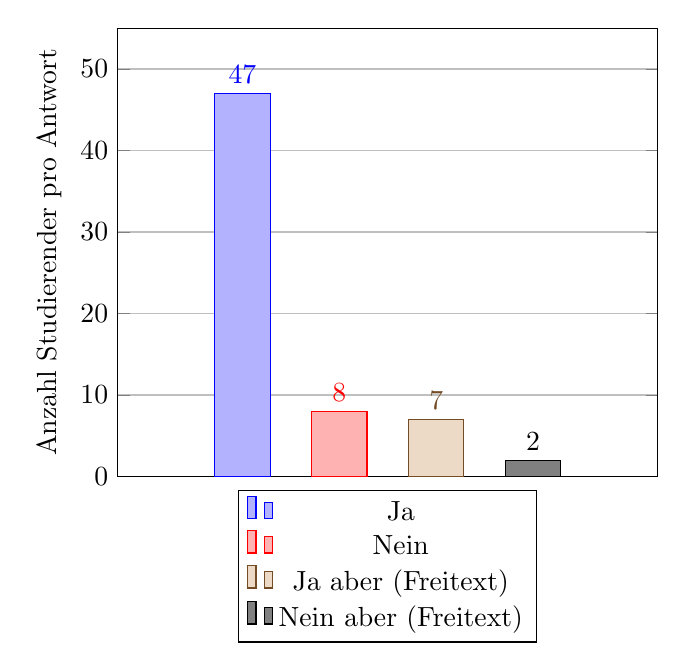
\begin{tikzpicture}
    \begin{axis}[
        x tick label style={
    		/pgf/number format/1000 sep=},
    	ylabel=Anzahl Studierender pro Antwort,
    	enlarge x limits=2,
        ymax=55,
        ymin=0,
    	legend style={at={(0.5,-0.03)},
        anchor=north,legend columns=1},
        ybar,
        bar width=20pt,
        xticklabels={},
        xtick=\empty,
        nodes near coords,
        grid=major,
    ]
    \addplot coordinates {(1,47)};
    \addplot coordinates {(2,8)};
    \addplot coordinates {(3,7)};
    \addplot coordinates {(4,2)};
    
    \legend{Ja, Nein, Ja aber (Freitext), Nein aber (Freitext)}
    \end{axis}
\end{tikzpicture}
    \caption{Grafische Darstellung der Ergebnisse zur Frage: Interessen an einem Lernsystem}
\end{figure}

Freitext: Ja, aber...
\begin{itemize}
    \setlength{\itemsep}{-1pt} 
    \item Nur falls ich es alleine nicht bereits checken sollte, sprich ich jetzt noch keine Erfahrung damit jemals gehabt hätte.
    \item Gamificationinhalte sollten dennoch eine gewissen Seriosität haben
    \item Es sollte generell standert in der lehre sein und ein einheitlciehs sytsem geben
    \item nur wenn auch tiefgehendere Lerninhalte vermittelt werden
    \item nur solange es nicht zu langatmig ist und die lernkurve steilgenug ist.
    \item Aktuell ist der Bedarf bei mir nicht mehr groß. Am Anfang des Studiums sehr gern
    \item es müsste Effizient wissen beibringen und meinen wissensstand berücksichtigen. sodass man nicht gelangweilt wird
\end{itemize}

Freitext: Nein, aber...
\begin{itemize}
    \setlength{\itemsep}{-1pt} 
    \item würde das System auch tiefgehende Konzepte umfassen, hätte ich durchaus Interesse
    \item hätte es evtl genutzt vor ein paar Jahren, als ich es gelernt hatte, wenn es zügig den Stoff behandelt.
\end{itemize}

\parbox{\linewidth}{
    Zum Schluss der Umfrage, wurde Teilnehmenden noch einmal die Möglichkeit gegeben, generelle Anmerkungen zur Umfrage oder zum Thema zu geben. Hierzu wurde ein einzelnes Freitextfeld bereitgestellt.

    \begin{itemize}
        \setlength{\itemsep}{-1pt} 
        \item Gamification für eine bessere Zukunft.
        \item Vielleicht ist für Anfänger auch wichtig zu verstehen, was anders an Git im Vergleich z.B. zu SVN oder Perforce/Helix Core ist.
        \item Etwas verwirrt hat mich, dass bei der Frage ``Git Kenntnisse'' das Verwenden von Branches auf die selbe Erfahrungsstufe gesetzt wird wie Git ``vollständig'' verstanden zu haben, wobei ich Branches eher bei den Git Grundlagen verordnen würde. Von daher war ich mir nicht ganz sicher wo ich mich auf der Skala einordnen soll
        \item Sollte unbedingt im Rahmen eines Pflichtkurs der Informatik eingehender behandelt werden. Mehr als, wie man ein commit macht, wurde leider nie erklärt. Ganz zu schweigen was ein Branch ist und wie man die handelt mit bspw. mehreren Projektteilnehmern.
        \item Ich finde es toll, dass eine Umfrage zu diesem Thema gemacht wird und hoffe, das Lernsystem zum Lernen von GIT noch kennenlernen zu dürfen. :)
        \item While I don't have a particularly deep understanding of git, I feel comfortable enough with my basic knowledge. So even though I rated my knowledge of git and GitHub rather low, it's always been enough for me.
    \end{itemize}
}

%
\include{content/chapDeclaration}
%
%
\end{document}